\documentclass[utf8,english]{gradu3}

\usepackage{graphicx}

\usepackage{amsmath}

\usepackage{booktabs}

% NOTE: This must be the last \usepackage in the whole document!
\usepackage[bookmarksopen,bookmarksnumbered,linktocpage]{hyperref}

\addbibresource{bibliography.bib} % The file name of your bibliography database

\begin{document}

\title{Using belief rule based systems for eliciting preference information in multiple criteria decision making problems (working title)}
\translatedtitle{Samma på Finska}
\studyline{Computer science}
\avainsanat{%n
    sääntöpohja,
    optimimointi,
    päätöksenteko,
    operatiivinen tutkimus,
  }
\keywords{
    rule based system,
    optimization,
    MCDM,
    operational research,
}
\tiivistelma{%
Liirum laarum.
}
\abstract{%
Lorem ipsum.
}

\author{Giovanni Misitano}
\contactinformation{\texttt{giovanni.a.misitano@jyu.fi}}
\supervisor{Jussi}
\supervisor{Kaisa}
\supervisor{Jian-bo?}

 % you don't need this line in a thesis
\type{Template and manual for a thesis document class}

\maketitle

\begin{thetermlist}
\item[\TeX] A batch-oriented typesetting system written by 
Donald Knuth in 1977--1989 \parencite[see][]{knuth86:_texbook}.
\end{thetermlist}

\mainmatter

\chapter{Introduction}
{\color{red}
Babbling, to be rewritten. Should contain a general introduction to the topic and motivation of this thesis.
}

When humans make decisions, it is natural to assume they know what they want.
This is reflected in many of the existing algorithms in multiple criteria decision making.
For example, in NIMBUS, it is assumed that the decision maker is capable of ranking how objectives
of a shown solution should change. Or in E-NAUTILUS, where the decision maker is asked to choose
a preferred point during each iteration. These algorithms are capable of aiding the decision maker to 
reach a preferred solution, and may even help the decision maker to learn something about the
underlying problem. However, these algorithms don't tell the decision maker much about
their preferences.

What if the preferences the decision maker gives do not match the preferences they
actually posses? Or what if the decision maker is not even sure what their preference is?

In this thesis, I will present a new method based on belief-rule based, systems to help a decision maker
the explore and learn about their preferences. The methods will be described in detail and will be tested in
practice in the form of a small case study. Based on the case study, the method will be assessed and
it will be discussed whether such method is practical and does it produce relevant information to a
decision maker.

This thesis is structured as follows. In chapter two through four, the underlying theory behind multiple
criteria decision making, multi-objective optimization and belief-rule based systems will be given. Chapter
five will contain a through description of the new model. Chapter six will present a case study in forest
management and will apply the developed model in real life practical setting. Chapter seven includes
discussions about the success of the case study. Finally, in chapter eight conclusions are made regarding
the new model and directions for further research are explored.

\section{Motivation}
{\color{red}
The general introduction to the topic behind this thesis, with a motivation driving the narration.
}

\section{Research questions}
{\color{red}
If I feel like stating the research questions explicitly.
}

\section{Previous research}
{\color{red}
This is where I touch on previous works that are relevant to this thesis. Relevance means, that the research has
used machine learning in trying to learn a DM's preference in a MCDM relevant context.
}

\section{Structure of this thesis}
{\color{red}
The general structure of this thesis is described.
}

\chapter{Optimization}

\section{Optimization}
\section{Why optimize?}
{\color{red}
What it is to optimize and why should we optimize? Some simple real-life examples.}
\section{Single-objective optimization}
{\color{red}
A formal, and general, presentation of a single-objective optimization problem.
}
\section{Multi-objective optimization}
{\color{red}
Like the previous section, but for MOO problems. A clear connection is made to the single-objective case. A real-life example is given to
introduce the reader to the topic, before the formalism (maybe in a separate sub-section before this section?)
}
\section{Pareto optimality}
{\color{red}
The concept of Pareto optimality is introduced, with a clear connection to MOO. It is also made clear what is meant by Pareto optimality in
this thesis.
}
\section{Solving optimization problems}
{\color{red}
Some methods for solving MOO problems are presented, with a focus on ASF. Brielfy describe a priori, a posteriori, and interactive methods.
Focus should be on interactive methods. Brief mention of evolutionary approaches, like NSGA. (mostly to show that the author is aware of other approaches.)
}

\chapter{Multiple criteria decision making}

\section{MCDM}
In this chapter, my aim is to introduce the reader to the concept of multiple criteria decision making in the
context of multi-objective optimization. Motivation, and an informal introduction to the 
central concepts, will be given in \ref{mcdmintro}. The following sections will dive deeper into the concepts, with
multi-objective optimization being presented in \ref{multiopt}. Methods for solving multi-objective optimization problems will be
presented in \ref{mcdmsolve}. In section \ref{mcdmdm} I will define what is meant by a decision maker, and how their preference
can be modelled. This chapter will conclude with section \ref{mcdminter} where I will explain what interactive methods are,
 why they are important, and I will reference methods in literature as examples of interactive methods.
 
The concepts presented in this chapter are fundamental to optimization. Various works can be found, such as \cite{Miettinen1998} and
\cite{yoshikazusawaragi1985}, to which I encourage the reader to refer to, if a more in-depth analysis of the presented concepts in this
chapter is desirable. My goal is to present a solid enough overview of the concepts in optimization that are relevant to this thesis.

\section{Introduction}
\label{mcdmintro}
A CEO of a multi-billion corporation has to decide what course to take, in terms of managing her business, in the
coming financial year to maximize the profit
of her corporation, and keeping the stake holders happy. A student is at his wit's end: Should he take a quickie
loan\footnote{A small loan that is quick and easy to get, but has a very high interest rate.}
to afford proper food, or should he swallow
his pride and fare with cup noodles for the rest of the month. A recruiter for a local supermarket has a couple of possible
candidates available for an open cashier job position: Who should the recruiter choose? The CEO, student, and recruiter, are
all very different people in very different situations, but what connects them, is that they are all trying to make
some decision.

In the previous scenarios, the CEO, student, and recruiter, are all in the position of a decision maker: They have
to make a decision based on the information available to them. The student, for example, has to decide whether to
take a small loan now to afford proper food, but with the increased cost of interests to be paid, or not to take a
loan, saving money, but having to cope with miserable food. It can be said, that the student has two objectives:
Minimizing his financial losses, and maximizing the quality of food. The student has also realized, to his knowledge or not,
that he cannot have gourmet food without paying a high cost, and he cannot pay pennies and expect a filet mignon. There is a
a trade-off between quality of food, and the money in his bank account; gaining in quality of food will lead to a loss
of capital, and trying to save money results in worse quality of food. It doesn't take much imagination to
imagine the CEO and the recruiter having to make similar trade-offs when deciding what to do.

This kind of decision making, where multiple criteria are conflicting, is at the heart multiple criteria decision making,
or MCDM in short. This thesis has a special focus on modelling the decision maker's behavior in a MCDM context. The concept
of preference also arises: Given a set of options, where no option can be traded to an other option without a loss in
some criteria, what option should a decision maker choose, and why did they choose that option? An underlying preference
guides the decision maker, and understanding this preference, can give insight into the logic of the decision maker,
which in turn, helps understand why the decision maker has made the decision he/she made.

\section{Optimization}
\label{multiopt}
In this section, my goal is to define what is meant by a multi-objective optimization problem. I will start by defining
a single-objective optimization problem in \ref{singleobj}, from which I will generalize the concepts to the concept of a multi-objective
optimization problem in \ref{multiobj}. Lastly, I will define concepts unique to multi-objective optimization problems in \ref{multiconcepts}.

The concepts presented in this chapter are fundamental to optimization. Various works can be found, such as \cite{Miettinen1998} and
\cite{yoshikazusawaragi1985}, which the reader is encourages to refer to, if a more in-depth analysis of the presented concepts in this
chapter is desired.

\subsection{Single-objective optimization}
\label{singleobj}
Before a multi-objective optimization problem can be formally defined, a general case of a single-objective optimization problem is
formulated. Based on this formulation, the formal definition of a multi-objective optimization problem, and related concepts, is
given later in this section.

In a single-objective optimization problem, an objective is usually defined as a scalar valued function of
one or multiple
independent variables. Both the function
and variables are real or integer valued. Formally, a single objective can be defined as

\begin{equation}
    \label{eq:objective}
    f: \mathbb{R}^n \to \mathbb{R},
\end{equation}

where $n$ denotes the number of dimensions in the domain of the objective function $f$, or in
other words, the number of variables the function is defined for.

The input variables, often called decision variables, for an objective function defined in \eqref{eq:objective},
can be defined as a vector
of independent variables, also called a decision variable vector:

\begin{equation}
    \label{eq:variablevector}
    \mathbf{x} = \Set{x_i \mid \forall i \in \left[1, n\right]},
\end{equation}

where $x_i$ denotes the value of the $i$th attribute. In the context of a single-objective optimization problem,
the variables of an objective function are often subject to constraints defined in the problem.
These constraints can be 
inequality constraints or equality constraints defined as:

\begin{equation}
    \label{eq:inequality}
    g_k: \mathbb{R}^{n_k} \to \mathbb{R}:\; g_k(\mathbf{x}) \leq 0,\quad\text{where}\;k\in\left[1, K\right],\;\text{and}\;n_k\leq n,
\end{equation}

and

\begin{equation}
    \label{eq:equality}
    h_l: \mathbb{R}^{n_l}\to\mathbb{R}:\;h_k(\mathbf{x}) = 0,\quad\text{where}\;l\in\left[1, L\right],\;\text{and}\;n_l\leq n.
\end{equation}

In \eqref{eq:inequality} and \eqref{eq:equality}, $K$ and $L$ denote, respectively,
the total number of that particular type of constraints present in the problem. The constraints in a single-objective
optimization problem define a certain feasible space for the variables $\mathbf{x}$, which can be denoted
as the feasible set $X$ of decision variable vectors. Therefore, the feasible decision variable vectors, of a single-objective
optimization problem, can be
denoted as

\begin{equation}
    \label{eq:feasibledecisionset}
    \mathbf{x} \in X \subseteq \mathbb{R}^n.
\end{equation}

In the case of $X=\mathbb{R}^n$ in \eqref{eq:feasibledecisionset}, the underlying optimization problem is said to be
unconstrained, where as in the case of $X\subset\mathbb{R}^n$, the problem is said to be constrained.

Based on the concepts defined so far, the full definition of a single-objective optimization problem can be given as

\begin{equation}
    \label{eq:singleobjectiveproblem}
    \max_{\mathbf{x}\in X} f(\mathbf{x}),
\end{equation}

where the objective function $f$ is to be maximized, and the decision variable vector $\mathbf{x}$ must be part of the feasible decision variable
vector space $X$. The choice of whether an objective function should be maximized or minimized, is arbitrary, but usually stems from the
nature of the objective in the optimization problem; profits are to be maximized, and losses are to be minimized. If need be, a maximization
problem can be transformed into a minimization problem by multiplying the objective by $-1$. For example, \eqref{eq:singleobjectiveproblem}
is equivalent to

\begin{equation}
    \label{eq:minussingleobjectiveproblem}
    \min_{\mathbf{x}\in X} -f(\mathbf{x}).
\end{equation}

The solution to a single-objective optimization problem is therefore defined as some $\mathbf{x^*}\in X$ which satisfies 
both \eqref{eq:singleobjectiveproblem} and \eqref{eq:minussingleobjectiveproblem}. The objective functions is said to reach its'
optimal value, when given $\mathbf{x^*}$ as argument.

In some cases there might be multiple solutions
to a single-objective optimization problem, for example in the case of minimizing the objective $f: \mathbb{R}\to\mathbb{R}:\;
f(x) = |x^2 - 1|$, both solutions
$x^*_1 = 1$ and $x^*_2 = -1$ minimize the function. In this case, the solutions $x^*_1$ and $x^*_2$
are considered to be equally preferable, meaning
there is no clear benefit\footnote{If there was a clear benefit in choosing one solution over the other,
it should be formulated in either the objective function of the problem,
or as a constraint of the problem.} in choosing one solution over the other.

\subsection{Multi-objective optimization}
\label{multiobj}
Like the name of this subsection suggests, in multi-objective optimization, the number of objectives to be optimized
is greater than one. These objectives are to be optimized, either minimized or maximized, simultaneously. The objective of a multi-objective
optimization problem can be either understood as a vector valued function, or as a set of multiple scalar valued functions. Formally,
and similarly to \eqref{singleobj}, the objectives of a multi-objective optimization problem can be expressed as

\begin{equation}
\label{eq:multiobj}
    \mathbf{f}: \mathbb{R}^n \to \mathbb{R}^M:\; \mathbf{f}(\mathbf{x}) = \Set{f_i(\mathbf{x})\mid\forall i \in [1, M]},
\end{equation}

where $M$ denotes the number of objectives, or the dimension of the objective space, in a multi-objective optimization
problem, and $f_i$ denote the components of the output of $\mathbf{f}$.
It's important to note that the decision variable vector $\mathbf{x}$ in \eqref{eq:multiobj} is the same for all
individual objective functions $f_i$. In this thesis, the objective of a multi-objective optimization problem is always understood
as a set of multiple scalar valued functions, each defined like \eqref{eq:objective}.

The constraint that define a feasible decision variable vector set in a multi-objective optimization problem, are defined equivalently
to \eqref{eq:equality} and \eqref{eq:inequality}, and the feasible space spanned is equivalent to \eqref{eq:feasibledecisionset}.
In other words, a multi-objective optimization problem is analogous to a single-objective optimization problem defined in 
\eqref{eq:singleobjectiveproblem} and \eqref{eq:minussingleobjectiveproblem}, but differs in the number of objectives.
Formally defined, a multi-objective optimization problem can be presented as

\begin{equation}
    \label{eq:multiobjectiveproblem}
    \max_{\mathbf{x}\in X} \mathbf{f}(\mathbf{x}) = \Set{f_i(\mathbf{x})\mid\forall i \in [1, M]},
\end{equation}

or

\begin{equation}
    \label{eq:minusmultiobjectiveproblem}
    -\min_{\mathbf{x}\in X} \mathbf{f}(\mathbf{x}) = \Set{f_i(\mathbf{x})\mid\forall i \in [1, M]}.
\end{equation}

However, defining a solution for a multi-objective optimization problem is not as straight forward as it was in the
case of a single-objective optimization problem.

\subsection{Central concepts in multi-objective optimization}
\label{multiconcepts}
The problem at the core of defining what can be considered to be a solution to a multi-objective optimization problem defined in
\eqref{eq:multiobjectiveproblem} and \eqref{eq:minussingleobjectiveproblem}, is that the objective function are seldom independent; the
objective function in a multi-objective optimization problem are in conflict\footnote{If the objective functions are
independent, then they can be optimized independently, and the optimal solution is optimal in regard to every objective function.}. This
means, that when one of the objective functions -- for the sake of argument, objective function $f_1$ -- 
attains its optimal value for some candidate solution $\mathbf{x}^*_1 \in X$,
it is very likely that some other objective function, $f_2$ for example, in the problem
does not attain its' optimal value. Then, choosing a new candidate solution $\mathbf{x}^*_2 \in X$, might result in $f_2$ reaching its'
optimal value, and for the objective function $f_1$ to steer away from its' optimal value in turn.

In a multi-objective optimization problem, a solution is not unambiguous, but rather, it is ambiguous, and the
concept of a single solution being optimal does not make sense. Therefore, the concept of a Pareto 
solution is defined.

The objective function value vector set is defined as

\begin{equation}
    \label{eq:objectivevalspace}
    Z = \mathbf{f}(X),
\end{equation}

and a feasible objective value vector is then any $\mathbf{z} \in Z$. Consider a
minimization problem, with $M$ objective functions,
and a feasible objective value vector $\mathbf{z}_i \in Z$.
$\mathbf{z}_i$  is a Pareto optimal solution if, and only if, no other solution $\mathbf{z}_j \in Z$
exists for which

\begin{equation}
    \label{eq:paretodef}
    \mathbf{z}_{j,k} \leq \mathbf{z}_{i,k}\;\forall\;k \in [1, M]
    \quad\text{and}\quad
    \mathbf{z}_{j,k} < \mathbf{z}_{i,k}\;\exists\;k \in [1, M]
    \quad\text{for all}\;\mathbf{z}_j\in Z \;\text{and}\; i\neq j
\end{equation}

is true. In \eqref{eq:paretodef} the index $k$ denotes the $k$th's objective function value. In other
words, \eqref{eq:paretodef} implies that no other objective value vector $\mathbf{z}_j$ exists in
$Z$, which has strictly better objective function values for all objectives. $\mathbf{z}_j$ must
therefore be worse at least in one objective function value when compared to $\mathbf{z}_i$.

The concept of a Pareto optimal solution can be extended to the concept of a  Pareto optimal set.
The Pareto optimal
set consists of all solutions $\mathbf{z}_i \in Z$, which satisfy condition \eqref{eq:paretodef}.
It follows that the Pareto optimal set $Z_{\text{Pareto}}$ is a proper subset of the feasible
objective function value vector set: $Z_{\text{Pareto}} \subseteq Z$.

Two other useful central concepts exists in multi-objective optimization. Namely, the ideal point, and
the nadir point. The ideal point $\mathbf{z}^*$ is defined as the objective function value vector
for a multi-objective optimization problem, where each of the objectives has been optimized
independently. The nadir point $\mathbf{z}_{\text{nad}}$
is defined similarly to the ideal point, but now the objective function
solution vector, representing the nadir point,
has a strictly worse value in each objective function compared to any feasible function
value vector in $Z$. The nadir point is ambiguous, and it is not as straight forward to compute as the
ideal point. It is beneficial to note that $\mathbf{z}^* \notin Z$, and $\mathbf{z}_{\text{nad}}
\notin Z$; the nadir and ideal points are not feasible objective function value vectors.

\begin{figure}[t]
    \centering
    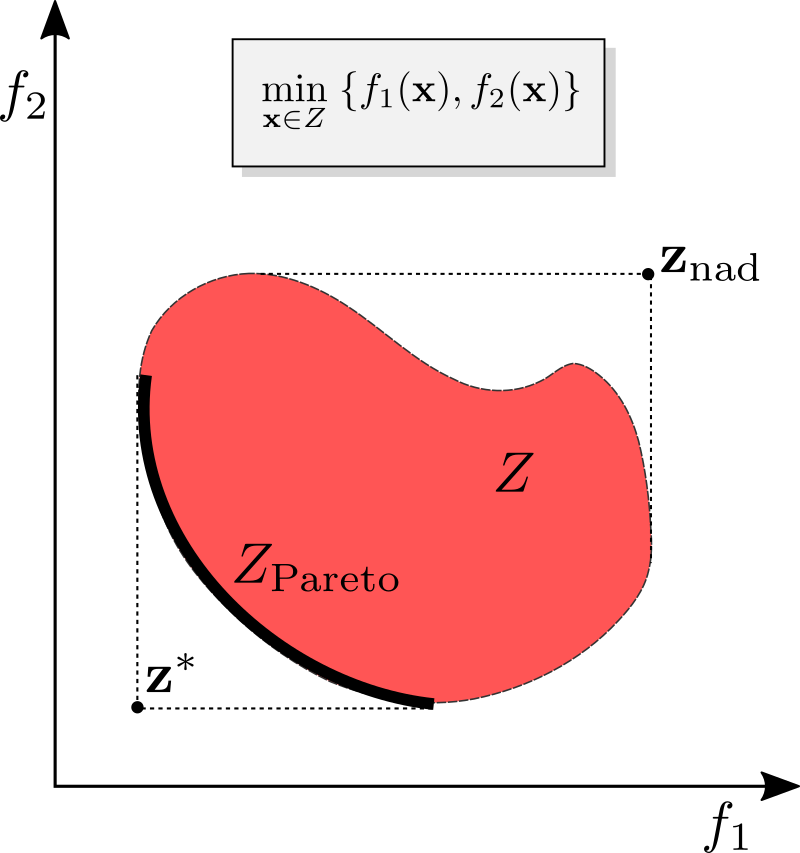
\includegraphics[width=8cm]{contents/moo_concepts.png}
    \caption{\emph{The central concepts of multi-objective optimization conceptualized graphically for a problem with two objectives. The objective function value vector set $Z$
    (filled area), the
    Pareto solution set $Z_{\text{Pareto}}$ (the thick line segment), the ideal point $\mathbf{z}^*$, and the nadir point $\mathbf{z}_{\text{nad}}$, are pictured.
    }}
    \label{fig:moo_concepts}
\end{figure}

The central concepts presented in this section have been conceptualized visually in figure \ref{fig:moo_concepts}
for a multi-objective optimization problem with two objective functions, that are to be minimized.
The Pareto optimal set in figure \ref{fig:moo_concepts} is convex, which is evident in the graphical continuity
of the line segments representing the Pareto optimal set. A non-convex Pareto optimal set would be graphically discontinuous.

\section{Solving multi-objective optimization problems}
\label{mcdmsolve}
{\color{red}
Solving multi-objective optimization problems, what is scalarization and what are ASFs.
}
Multi-objective optimization problems are not straight forward to solve, because the solution is not unambiguous. Without
any kind of preference information, it is impossible in a Pareto optimal set to say that one solution is better than the other.
The number of possible Pareto optimal solution can also be very large, even uncountable, which poses its' own challenges: How many
Pareto optimal solutions should be solved for? Should the Pareto optimal set be evenly distributed? Is some region of the Pareto optimal
set more preferable than others? This section presents methods for solving multi-objective optimization methods by means of scalarization.
A brief overview of other existing methods is also given, and references to the methods described are provided.

\subsection{A word on solving single-objective optimization problems}
\label{solvingsingle}
The crucial methods for solving multi-objective optimization problems, relevant to this thesis, boil down to solving
single-objective optimization problem(s), that capture some sort of given preference, which is defined in section \ref{mcdmdm},
and produce a
solution to the original multi-objective optimization problem, which in turn, reflects the given preference. That is why this chapter
starts with a brief discussion about how to solve single-objective optimization problems.

To solve the single-objective optimization problem, it is necessary to find a solution
$\mathbf{x} \in X$ that minimizes \eqref{eq:singleobjectiveproblem}, or maximizes \eqref{eq:minussingleobjectiveproblem}. 
Various methods exist in literature to solve for $\mathbf{x}$.
Examples of typical, and straightforward, methods are the simplex method,
and Newton's method, which are both -- and accompanied by many more similar methods --
presented in \cite[chapter 9 and 10]{williampress2007}, all paired by blueprints for implementing them in software code.

However, relevant to this thesis, two methods emerge: sequential least squares programming (SLSQP) \cite[chapter 10]{jorgenocedal2006},
and Coin-or branch and cut (CBC) \cite{zenodo2018}. SLSQP is very versatile: it is able to solve non-linear constrained single-objective 
optimization problems. When training belief rule-based system, as discussed in section \ref{training}, the emerging problem to be
solved is a single-objective constrained non-linear optimization problem, which SLSQP is able to solve.

CBC is suitable for solving mixed integer problems: problems were the decision vector variables have real and integer valued
elements. Therefore, CBC is suitable for solving the emerging achievement scalariztion functions, when solving for the Pareto optimal set
in the Finnish forestation case study discussed in section \ref{finnishforestation}.

This subsection will not delve further into the details of each method. For the rest of this section, it is assumed that a method
for solving constrained non-linear single-objective optimization problems exists.

\subsection{Scalarization}
The vector valued objective function present in multi-objective optimization problems \ref{eq:multiobjectiveproblem}, can be transformed
into a vector valued function using some scalarizing function transformation:

\begin{equation}
    \label{eq:funstransform}
    \mathbf{f}: \mathbb{R}^n \to \mathbb{R}^M \;\xrightarrow{{\text{scalarization}}}\; f: \mathbb{R}^n \to \mathbb{R}.
\end{equation}

Therefore, the multi-objective optimization problem is reduced to a single-objective optimization problem, which can be solved using
methods discussed in \ref{solvingsingle}.

As an example, the weighting method transforms the multi-objective optimization problem \ref{eq:multiobjectiveproblem}
into the single-objective problem

\begin{equation}
    \label{eq:weighting}
    \max_{\mathbf{x} \in X} \sum_{i=1}^{M} w_i f_i(\mathbf{x}) \; ,\quad\text{where}\;\sum_{i=1}^{M}w_i = 1\;\text{and}\;w_i \ge 0\;\forall i\in [1, M].
\end{equation}

In problem \eqref{eq:weighting}, $w_i$ are weights associated to the $i$th objective function in the original multi-objective optimization problem. It is proven in
\cite[chapter 3.1]{Miettinen1998}, that when the solution to \ref{eq:weighting} is found, it is Pareto optimal, if the weights $w_i$ are all positive, and the solution
found is unique.

The weighting method is able to produce different Pareto solutions with a different choice of weights. However, there are limitations to the extent of
its' ability to produce Pareto optimal solutions. If the underlying Pareto optimal set is non-convex, the weighting method cannot find all the
solutions\cite[chapter 3.1]{Miettinen1998}. See also \cite{Das1997} for further criticism on generating Pareto optimal solution sets using weighted
sums.

Therefore, the main merit of the weighting method is in its' simplicity, and ease of implementation.
An overview
of other existing scalarization functions can be found in \cite{Coello2017}.

\subsection{Achievement scalarizing functions}
\label{asf}
Achievement scalarizing functions are a set of scalarization function to scalarize multi-objective optimization problems. Achievement scalarizing function are
scalar valued functions of the form

\begin{equation}
    \label{eq:asf}
    s_{\mathbf{\bar{z}}}: \mathbb{R}^M \to \mathbb{R}:\;s_{\mathbf{\bar{z}}}(\mathbf{z}) = s_{\mathbf{\bar{z}}}(\mathbf{f(\mathbf{x}})),
\end{equation}

where $\mathbf{\bar{z}} \in \mathbb{R}^M$ is a reference point, and $\mathbf{f}$ is the objective function of a multi-objective optimization problem
\ref{eq:multiobjectiveproblem}. Using an achievement scalarizing function, an achievement problem

\begin{equation}
    \label{eq:asfproblem}
    \min_{\mathbf{z}\in Z}\; s_{\mathbf{\bar{z}}}(\mathbf{z})
\end{equation}

can be formulated. It is proven in \cite[chapter 3.5]{Miettinen1998}, that when \eqref{eq:asf} is increasing, and the solution to the achievement problem
is unique, then the solution is Pareto optimal. For solving \eqref{eq:asfproblem}, it is required to find an objective vector $\mathbf{z}$, which minimizes
\eqref{eq:asfproblem}. Methods discussed in \ref{mcdmsolve}, are suitable for solving achievement problems as well.

In the case study discussed in \ref{casestudy}, a Pareto optimal set is generated using an achievement scalarizing function, which will be
referred to as the guess function, used in the
GUESS method \cite{Buchanan1997}

\begin{equation}
    \label{eq:guessasf}
    s_\mathbf{\bar{z}}(\mathbf{z}) = \max_{i \in [1, M]}
    \left[ \frac{z_i - z_i^{\text{nad}}}
    {z_i^{\text{nad}} - \bar{z}_i}
    \right],
\end{equation}

where $z_i$ and $\bar{z}_i$ are the components of the objective value vector $\mathbf{z}$ and $\mathbf{\bar{z}}$ respectively. Intuitively,
the guess function, when minimized, results in a Pareto optimal objective value vector $\mathbf{z}$, which has components $z_i$ that have the minimized maximum
deviation, in each component, compared to the nadir point, and which resides on a line segment connecting the reference point and the nadir point.
This is a very straight forward way of calculating a Pareto optimal solution, with minimal assumptions made. Only the nadir point of the original
multi-objective optimization problem is required, and the reference point chosen must be smaller\footnote{Or bigger, if maximization is desired in the
underlying multi-objective optimization problem.}
in every component compared to the nadir point.
How to generate nadir points will be discussed later. In
\cite[chapter 5.7]{Miettinen1998}, it is shown that any Pareto optimal solution can be found when using the guess function.

The guess function can be used to generate a representation of a Pareto optimal set, for a multi-objective optimization problem, by
generating a set of reference points, and solving the achievement scalarizing problem \eqref{eq:asfproblem} using the guess function.
This method of solving for the Pareto optimal set is somewhat similar to the the normal-boundary intersection method \cite{Das1998},
where a set of reference points is also generated, but the analytical form of the objective functions must be
available\footnote{The problem must be either formulated mathematically, or some  surrogate model modelling the
objective functions must be available.}, which is not the case when using an achievement scalarization function.
The guess function has also the advantage to
not suffer from the same limitations as the weighted method \eqref{eq:weighting} mentioned earlier.

Examples of other available achievement scalarization functions, and their comparisons, can be found in \cite{Miettinen2002}.

\section{The decision maker and preference}
\label{mcdmdm}
{\color{red}
What is meant by a decision maker and what is their role. Preference as a concept and utility functions as a model of that concept.
}

So far, only the optimization aspect of multiple criteria decision making has been discussed. This section presents the concept of a decision maker,
and preference, which are in a central role in multiple criteria decision making.

\subsection{The decision maker}
In the context on multiple criteria decision making, the decision maker is usually a human, who is an expert in some field.
The decision maker can be singular, or it can be a group of decision makers. When a group of decision makers is in question,
it is referred to as group decision making. The decision maker can also be artificial, for example an expert system. However,
in the scope of this thesis, only the case of a decision maker, consisting of a single human expert, is of concern.

The role of the decision maker is that of providing preference information, which is not evident
from the general formulation of a multi-objective optimization problems. Preference information can be given by the decision maker
in different forms, and at different times, when solving a multi-objective optimization problem.

When preference is given before a multi-objective optimization problem is solved, preference is said to be given a priori. When preference is
given after a Pareto optimal set has been solved for a multi-objective optimization problem, preference is said to be given a posteriori.
Preference can also be given interactively, which means it is given during the process of solving a multi-objective optimization problem.
Different methods for solving multi-objective optimization problems are usually classified using these three terms: a priori methods,
a posteriori methods, and interactive methods.


\section{Interactivity}
\label{mcdminter}
{\color{red}
Interactivity in MCDM problems, what is meant and why.
}

\chapter{Belief rule-base systems}

\section{Belief rule-base}
I will begin this chapter with a less formal introduction to traditional rules and rule sets given in \ref{rulesandrulesets}.
Following it, I will go into more detail of belief rule-based systems giving a more formal presentation in \ref{TODO}.

\section{Rules and rule sets}

{\color{red}I hope this sort of informal introduction giving an intuitive introduction to the main topic to be discussed
is appropriate in a thesis. I would skip this in a journal article.}

\label{rulesandrulesets}
Rules are a natural way of conveying information on how an agent or system should work according to its' surrounding environment.
A rule can be as simple as an if... then... statement; such a rule could be for example:

\begin{displayquote}
\textbf{Rule 1:} ``\textit{If it rains outside, bring an umbrella.}``.
\end{displayquote}

%However, such rules are strict. What if Bob is not sure if it is going to rain? Should he still take an umbrella if the sky looks dark?
%Belief-rule based systems are meant to tackle such scenarios. They extend the idea of rules to include a certain degree of belief to each rule.
%Then, given an observation, such as, how dark the sky looks, a belief-rule based system can give an answer that Bob should probably bring an umbrella,
%if he decides to venture outside.
A rule consists of three elements: the precedent, the condition, and the consequent. Take rule 1 as an example.
Suppose there was an agent named Bob who is contemplating whether he should bring an umbrella
outside or not. The precedent in the example should give a definite answer to the question implied by the condition of
the rule "if it rains". The question implied is "Does it rain?".
Therefore, Bob needs to look outside and see if it rains or not; he needs information from the surrounding environment.
Using the observed precedent and the condition, the rule can be resolved: If bob observes rain, he 
should bring an umbrella outside.

However, the rule in the previous example does not state anything
regarding the case when it does not rain outside. One could argue that the rule implicitly suggests to not bring an umbrella
in the absence of rain,
but it is not an explicit consequent of the rule in the case of no rain. To cover the case of no rain,
an additional rule should be stated:

\begin{displayquote}
\textbf{Rule 2:} ``\textit{If it does not rain outside, do not bring an umbrella.}``.
\end{displayquote}

In turn, rule 2 does not state anything regarding the case when it does rain outside. 
For Bob to have a coherent set of actions to take, whether to bring an umbrella outside or not,
the rules 1 and 2 should be combined into a single rule set:

\begin{displayquote}
\textbf{Rule set 1:}
\begin{cases}
``\textit{If it rains outside, bring an umbrella.}`` \\
``\textit{If it does not rain outside, do not bring an umbrella.}`` 
\end{cases}
\end{displayquote}

Rule set 1 is now a complete rule set; a definite consequent follows all possible precedents, namely "It rains outside."
and "It does not rain outside.". If there was a third precedent in the example, for example: "It might be raining outside", rule set 1
would be incomplete and is said to contain a degree of ignorance: It does not state what to do in the case when the observation of rain
is indefinite.

That being said, in real life, observations are seldom definitive. To cover all possible cases of
different observations, made by Bob in rule set 1,
would mean an addition of an indefinite number of rules, with the precedents covering all possible cases.
In practice, trying to cover all cases is an exercise in futility.

Could the conditions of rules in a rule set have a degree of truthiness associated to them, instead of being simply true of false?
Could such rule set cover a continuous range of observations and outcomes?
Is it possible to infer an appropriate consequent from such a rule set, and how to interpret the outcome?
This is where belief rule-based systems come into play.

\section{Belief rules}
In a belief rule $R$, the precedent is defined as a set of finite arrays of referential values, and the consequent
is defined as a single finite array of referential values. In this thesis, it is assumed that these referential values
are real numbers.

Following the RIMER approach \cite{rimer2006} to define a belief rule,
a referential array set $A$, called a packet precedent, with finite arrays $A_i$, is defined as the precedent of a 
belief rule:

\begin{equation}
\label{eq:A_set_def}
    A = \Set{ A_i = \Set{A_{i, n} \mid \forall n \in \left[1, \left|A_i\right| \right]}
    \mid \forall i \in \left[1, T \right] }, \quad\text{where}\quad i, n, T \in \mathbb{N}.
\end{equation}

And an array of finite values, $D$, is defined as the consequent in a belief rule:

\begin{equation}
\label{D_set_def}
    D = \Set{D_j \mid \forall j \in \left[1, N \right] }, \quad\text{where}\quad j, N \in \mathbb{N}.
\end{equation}

In \eqref{A_set_def} and \eqref{D_set_def}, $T$ is the total number of attributes in an observation, $A_i$ is the array of possible  referential values
for the $i$th attribute in an observation, $\left|A_i\right|$ is the number of referential values for the $i$th attribute in an observation,
and $N$ represent the total number of referential values for the consequent.

The input to a belief rule is defined as an observation $X$, which is an array of observed precedent values
for $T$ attributes defined as

\begin{equation}
    \label{eq:X_input}
    X = \Set{ x_i \mid \forall i \in \left[1, T \right]}, \quad\text{where}\quad i \in \mathbb{N}.
\end{equation}

The values $x_i$ in \eqref{eq:X_input} take values equal to the finite arrays $A_i$ present in the packet
antecedent $A$ in \eqref{eq:A_set_def}.

The condition of a belief rule can be defined as a logical relationship $F$ between the observation $X$, and
the packet antecedent $A$ as

\begin{equation}
    \label{eq:logical}
    F : x_1\;\text{is}\;A_1\;\land\;x_2\;\text{is}\;A_2\;\land\dots\land\;x_T\;\text{is}\;A_T.
\end{equation}

The logical relation $\land$ present in \eqref{eq:logical}, could be replaced by some other logical relation, but in this thesis,
the RIMER approach is followed, which uses the $\land$ relation.

Finally, a real valued belief degree $\beta_j$ can be defined for a belief rule. $\beta_j$ represents the degree of belief for $D_j$ to be the consequent
in a belief rule, when $F$ is given.

Therefore, a single belief rule can be defined as

\begin{equation}
\label{singlerule}
    \tilde{R} = \braket{X, A, D, F}{}.
\end{equation}

The single rule \eqref{singlerule} can be then be generalized to a finite set of $L \in \mathbb{N}$ belief rules as

\begin{equation}
    R = \Set{ \braket{X, A^k, D, F_k} \mid k \in \left[1, L \right]},
\end{equation}

which is understood as each rule $R_k$ having its' own set of referential value arrays $A^k$, and a logical relationship $F_k$, but the same observation $X$, and
the same consequent referential values $D$.

%For a real valued observation $X$ to be usable with a belief rule, the observation must be first expressed as a belief distribution over
%the set of referential values defined for the precedents in the rule. It is therefore assumed that $A$ is defined in a way, which allows the expression
%of the observation $X$. As presented in \ref{TODO}, the observation $X$ can be transformed to the following distribution

%\begin{equation}
%    \alpha = \Set{
%    \min{\left(
%    \max{\left( \frac{A_{i+1} - X}{A_{i+1} - A_{i}}, 0 \right)},\:
%    \max{\left( \frac{X - A_{i-1}}{A_i - A_{i-1}}, 0 \right)}
%    \right)}
%    \mid \forall i \in \left[1, T\right] },
%\end{equation}

%where $A_0 = A_T$ and $A_{T+1} = A_1$.

\section{Handling uncertain information}
{\color{red}
Belief distributions and belief degrees are presented, and the link to belief rules is established.
}

\section{Belief rule-base systems}
{\color{red}
Aggregates the previous two sections into one coherent entity, finally giving a formal representation of a BRB model.
}

\section{Inference on belief rule-base systems}
{\color{red}
How to use evidential reasoning to reason about a BRB system. Formulas are shown, not derived, on how to transform an input to a BRB system,
how to calculate activation weights of
a BRB system using the transformed input, and how the belief degrees can then be calculated using the activation weights. What is a belief rule expression matrix?
}

\section{Training belief rule-base systems}
{\color{red}
The concept of an initial principle to build an initial belief rule expression matrix.
The tunable parameters of a BRB system are briefly explored. It is then explained how these parameters can be tuned using known information of
a system that is to be modelled.
}

\section{Transparency of belief rule-base systems}
{\color{red}
Observation of the transparency of the model combined to its' adaptive nature makes it a good candidate as an explainable machine learning tool.
}

\section{Belief rule-base systems as machine learning models}
{\color{red}
Why BRBs are good candidates of ML models? References to real life applications are given as a motivation. Suggest BRBs to have above average explainability,
compared to blackbox models, such as deep neural networks.
}

\section{Examples}
{\color{red}
Finally, a simple numerical example is given, with a link to the source code to reproduce the results. I plan to model a non-linear function, and show,
the capability of a BRB system in modelling a non-linear system as a motivation. It is mentioned that the author has developed a simple software library to implement
trainable BRB models.
}

\section{Evidential reasoning}
\input{contents/evidential.tex}

\chapter{Case study}
\section{Motivation}
{\color{red}
Why have a case study?
}

\section{Problem in Finnish forestation}
{\color{red}
Present the problem used in the case study being formal where needed. The MOO and MCDM  part of the problem should be formalized the framework laid in
previous chapters. Describe the used data, how it has been modified (engineered), and give reference to data used in this thesis.
}

\section{Solving for the Pareto front}
{\color{red}
How the Pareto front has been solved using an ASF. Extent of the Pareto front is discussed, and assumptions regarding the front are made clear.
Related source code, for solving the Pareto front, is referenced
}

\section{Eliciting the decision maker's preferences}
{\color{red}
How the method described in chapter 5 has been used.
}

\section{Results}
{\color{red}
Results of using the method described in chapter 5 to elicit the DM's preference model.
}

\chapter{Discussion}
\section{Success in eliciting a decision maker's preference model}
{\color{red}
What went right, what went wrong. Did we end up with a model that can model a DM's preference? How to assess this?
}

\section{Comparing the method and results to existing work}
{\color{red}
Brief look into related works, where it is attempted to model a DM's preference model using some sort of machine learning.
}

\section{Viability and suggestions for related research topics}
{\color{red}
Is the developed method viable, should future research stem out of it? If so, what kind of reserach should be pursued? What was left open to research in this
thesis?
}

\chapter{Conclusion}
\section{Epitome}
{\color{red}
Wrap up of what has been done, the main results, and where to go next. Were the research questions answered, and what
are the final answers?
}

\section{Acknowledgements}
{\color{red}
Acknowledgements as deemed necessary.
}

\printbibliography

\appendix
{\color{red}
Expanded as the need raises.
}

\end{document}
